\chapter{نتایج}
\section{معیارهای ارزیابی در یادگیری عمیق}

در این بخش، به بررسی معیارهای مختلفی که برای ارزیابی مدل‌های یادگیری عمیق استفاده می‌شوند، می‌پردازیم. این معیارها شامل \lr{Sensitivity}، \lr{Specificity}، \lr{Precision}، \lr{F1 Score}، \lr{Accuracy}، \lr{Intersection over Union (IoU)} و ضریب \lr{Dice} است.

قبل از پرداختن به تعریف این معیارها، ابتدا به تعریف چهار مفهوم اساسی می‌پردازیم که در فرمول‌های ارزیابی به ‌کار می‌روند:

\begin{itemize}
    \item \textbf{\lr{TP} \lr{(True Positives)}}: تعداد نمونه‌های مثبت که به‌درستی به‌عنوان مثبت دسته‌بندی شده‌اند.
    \item \textbf{\lr{FP} \lr{(False Positives)}}: تعداد نمونه‌های منفی که به‌اشتباه به‌عنوان مثبت دسته‌بندی شده‌اند.
    \item \textbf{\lr{TN} \lr{(True Negatives)}}: تعداد نمونه‌های منفی که به‌درستی به‌عنوان منفی دسته‌بندی شده‌اند.
    \item \textbf{\lr{FN} \lr{(False Negatives)}}: تعداد نمونه‌های مثبت که به‌اشتباه به‌عنوان منفی دسته‌بندی شده‌اند.
\end{itemize}

\subsection{\lr{Sensitivity}}

\lr{Sensitivity}
که با نام نرخ تشخیص صحیح نیز شناخته می‌شود، معیاری برای ارزیابی توانایی مدل در تشخیص صحیح نمونه‌های مثبت است. فرمول این معیار در \autoref{eq:sensitivity} مشخص شده است.

\begin{latin}
\begin{equation}
\label{eq:sensitivity}
\text{Sensitivity} = \frac{TP}{TP + FN}
\end{equation}
\end{latin}

\subsection{\lr{Specificity}}

\lr{Specificity}
، معیاری است که نشان‌دهنده توانایی مدل در شناسایی صحیح نمونه‌های منفی است. فرمول این معیار در \autoref{eq:specificity} مشخص شده است.

\begin{latin}
\begin{equation}
\label{eq:specificity}
\text{Specificity} = \frac{TN}{TN + FP}
\end{equation}
\end{latin}

\subsection{\lr{Precision}}

\lr{Precision}،
 معیاری برای ارزیابی میزان درستی دسته‌بندی نمونه‌های مثبت است.به‌عبارت‌دیگر،
  \lr{Precision}
   نسبت نمونه‌های مثبت درست دسته‌بندی شده به تمام نمونه‌های پیش‌بینی‌شده به‌عنوان مثبت است. فرمول آن در
    \autoref{eq:precision}
     مشخص شده است.

\begin{latin}
\begin{equation}
\label{eq:precision}
\text{Precision} = \frac{TP}{TP + FP}
\end{equation}
\end{latin}

\subsection{\lr{F1 Score}}

\lr{F1 Score}، میانگین موزون \lr{Precision} و \lr{Sensitivity} است که تعادلی بین این دو معیار ایجاد می‌کند. این امتیاز به‌ویژه در مواردی که تعادل بین \lr{Precision} و \lr{Sensitivity} اهمیت دارد، مورداستفاده قرار می‌گیرد. فرمول \lr{F1 Score} در \autoref{eq:f1_score} مشخص شده است.

\begin{latin}
\begin{equation}
\label{eq:f1_score}
\text{F1 Score} = 2 \times \frac{\text{Precision} \times \text{Sensitivity}}{\text{Precision} + \text{Sensitivity}}
\end{equation}
\end{latin}

\subsection{\lr{Accuracy}}

\lr{Accuracy}، نسبت نمونه‌هایی است که به‌درستی دسته‌بندی شده‌اند به تمام نمونه‌ها. این معیار نشان‌دهنده عملکرد کلی مدل است و فرمول آن در \autoref{eq:accuracy} مشخص شده است.

\begin{latin}
\begin{equation}
\label{eq:accuracy}
\text{Accuracy} = \frac{TP + TN}{TP + TN + FP + FN}
\end{equation}
\end{latin}

\subsection{\lr{Intersection over Union (IoU)}}

\lr{Intersection over Union}
 که به‌عنوان \lr{Jaccard Index} نیز شناخته می‌شود، معیاری است که برای ارزیابی همپوشانی بین دو مجموعه، به‌ویژه در مسائل بخش‌بندی تصویر، استفاده می‌شود. فرمول \lr{IoU} در \autoref{eq:iou} مشخص شده است.

\begin{latin}
\begin{equation}
\label{eq:iou}
\text{IoU} = \frac{|A \cap B|}{|A \cup B|} = \frac{TP}{TP + FP + FN}
\end{equation}
\end{latin}

\subsection{ضریب
\lr{Dice}}

ضریب \lr{Dice}، مشابه \lr{IoU} است؛ اما وزن بیشتری به ناحیه اشتراک می‌دهد و در مسائل بخش‌بندی تصویر بسیار مورداستفاده قرار می‌گیرد. فرمول ضریب \lr{Dice} در \autoref{eq:dice} مشخص شده است.

\begin{latin}
\begin{equation}
\label{eq:dice}
\text{Dice Coefficient} = \frac{2 \times |A \cap B|}{|A| + |B|} = \frac{2 \times TP}{2 \times TP + FP + FN}
\end{equation}
\end{latin}

\section{نتایج طبقه‌بندی}

در این بخش، نتایج حاصل از مدل‌های طبقه‌بندی خونریزی درون‌جمجمه‌ای در تصاویر سی‌تی‌اسکن، بررسی و تحلیل شده‌اند. تمرکز اصلی آموزش مدر طبقه‌بندی بر روی بهینه‌سازی فراپارامترها برای مدل
 \lr{ResNet50}
  بوده است که بهبود قابل‌توجهی در عملکرد مدل به‌ویژه در معیار \lr{Sensitivity}
   به ‌همراه داشته است. بهترین نتایج به‌دست‌آمده در جستجوی شبکه‌ای زمانی حاصل می‌شود که ضریب افزایش مصنوعی داده برابر 
   $3.3$
و وزن تابع خطا
\lr{Cross-entropy}
برای برش‌های مثبت برابر 4 و برای برش‌های منفی برابر 1 است.

\subsection{نتایج برش‌محور }
پس از آموزش مدل طبقه‌بندی برای تمام 
\lr{Fold}ها،
نمودار امتیاز
\lr{F1}
نسبت‌ به آستانه‌های متفاوت رسم شد و در گام بعدی میانگین این نمودارها محاسبه شد. در انتها بهترین آستانه روی میانگین این نمودار‌ها محاسبه شده و در محاسبه معیارهای مربوط به زیرمجموعه ارزیابی استفاده شده است.
 \autoref{tab:slice_level_results}
  نتایج به‌دست‌آمده از آموزش مدل‌های \lr{ResNet50} و سازوکار شورا برای طبقه‌بندی برش‌محور نشان می‌دهد. همان‌طور که در جدول مشاهده می‌شود، بهترین نتایج در
 \lr{Fold 0}
  به‌دست‌آمده است که امتیاز 
  \lr{F1}
   برابر با
  $0.62$
 را نشان می‌دهد. این نشان‌دهنده این است که توزیع داده‌ها در مجموعه‌های آموزشی و اعتبارسنجی این 
 \lr{Fold}
  بیشتر شبیه به مجموعه آزمون است. در مقابل، 
  \lr{Fold 4}
   کمترین نتایج را به‌دست‌آورده، درحالی‌که نتایج مراحل دیگر با هم بیشتر هم‌خوانی دارند. نتایج به‌دست‌آمده از روش شورایی، در مقایسه با نتایج گزارش‌شده توسط
   \lr{Hssayeni}\cite{hssayeni2020intracranial}
   و همکاران، در معیار
   \lr{Sensitivity}
3 درصد ضعیف‌تر عمل کرده ‌است اما در معیار
\lr{Specifity}
41 درصد بهتر عمل کرده است. مقایسه این نتایج نشان می‌دهد که مدل پیشنهادی در این پژوهش، به‌صورت نسبی همان قدر که در تشخیص برش‌هایی که خونریزی درون‌جمجمه‌ای دارند درست عمل می‌کند، در تشخیص برش‌هایی که سالم هستند نیز درست عمل می‌‌کند اما 
\lr{Hssayeni}
و همکاران در تشخیص برش‌های سالم که تعداد آنها نیز بسیار زیاد هست،‌ ضعیف عمل کرده‌اند و 50درصد از این برش‌ها را دارای خونریزی درون‌جمجمه‌ای تشخیص داده‌اند. نکته‌ای که در مورد پژوهش آنها وجود دارد،‌ عدم ارائه بقیه معیارهای ارزیابی مدل است که تحلیل و مقایسه‌ بیشتر این پژوهش را دشوار می‌سازد.
پژوهش بعدی که در زمینه طبقه‌بندی برش‌های خونریزی درون‌جمجمه‌ای با استفاده از انتقال یادگیری عمل کرده است، مربوط به 
\lr{Neethi}\cite{neethi2022stroke}
است که از مدل 
\lr{ResNet 50} 
استفاده کرده‌اند. این پژوهش در معیار
\lr{Precision}
20 درصد و در معیار امتیاز
\lr{F1}
3 درصد بهتر عمل کرده ‌است اما در معیار 
\lr{Sensitivity}
مدل آنها 18 درصد ضعیف‌تر و در معیار 
\lr{Accuracy}
مدل آنها 37 درصد ضعیف‌تر عمل کرده است. در تحلیل نتایج به‌دست‌آمده، از‌آنجایی‌که در زمینه پزشکی، تشخیص اشتباه یک نمونه دارای بیماری،‌ می‌تواند منجر به حوادث جبران‌ناپذیر شود، معیار 
\lr{Sensitivity}
مهم‌تر از معیار 
\lr{Precision}
است؛ باتوجه‌به این نکته،‌ مدل پیشنهادی ما توانسته اختلاف بسیار زیادی در این معیار ایجاد کند. از طرف دیگر با‌توجه‌به عدد 
\lr{Accuracy}
گزارش شده، مشخص است که مدل پیشنهادی 
\lr{Neethi}
تنها نیمی از برش‌های تمام مجموعه‌داده را درست تشخیص داده که نشان‌دهنده تعداد خیلی کم 
\lr{TN}
و مقدار کم 
\lr{Specificity}
است که در پژوهش آنها گزارش نشده است. نکته‌ای که باید توجه داشت این است که مدل‌های استفاده شده در هر دو پژوهش یکسان است و تنها فراپارامتر‌های پیشنهادی ما باعث بهبود عملکرد مدل شده است.


% Please add the following required packages to your document preamble:
% \usepackage{graphicx}
\begin{table}[h]
\centering
\caption{نتایج برش‌محور مدل \lr{ResNet50}
برای آستانه تصمیم‌گیری
$0.27$}
\label{tab:slice_level_results}
\resizebox{\textwidth}{!}{%
\begin{tabular}{llllll}
\hline
\multicolumn{1}{c}{\textbf{مدل}}           & \textbf{\lr{Sensitivity}} & \textbf{\lr{Specificity}} & \textbf{\lr{Precision}} & \textbf{\lr{F1}}   & \textbf{\lr{Accuracy}} \\ \hline
\lr{ResNet50 Fold 0}        & $0.78$            & $0.93$             & $0.51$         & $0.62$ & $0.91$    \\
\lr{ResNet50 Fold 1}        & $0.68$            & $0.90$             & $0.38$         & $0.49$ & $0.88$    \\
\lr{ResNet50 Fold 2}        & $0.60$            & $0.89$             & $0.33$         & $0.42$ & $0.86$    \\
\lr{ResNet50 Fold 3}        & $0.86$            & $0.89$             & $0.41$         & $0.55$ & $0.89$    \\
\lr{ResNet50 Fold 4}        & $0.32$            & $\mathbf{0.96}$             & $0.42$         & $0.36$ & $0.90$    \\ \hline
\lr{Neethi et al.}\cite{neethi2022stroke} & $0.76$            & $-$                & $\mathbf{0.69}$         & $\mathbf{0.67}$ & $0.54$    \\
\lr{Hssayeni et al.}\cite{hssayeni2020intracranial}                & $0.97$               & $0.50$                & $-$            & $-$    & $-$       \\ \hline
\lr{ResNet50} شورایی        & $\mathbf{0.94}$            & $0.91$             & $0.49$         & $0.64$ & $\mathbf{0.91}$   
\\ \hline
\end{tabular}%
}
\end{table}



همان‌طور که در 
\autoref{fig:ch3-f1-vs-th-cls}
 مشاهده می‌شود، با استفاده از سازوکار شورایی، امتیاز \lr{F1} بهبود قابل‌توجهی پیدا کرده است که نشان‌دهنده بهبود عملکرد مدل طبقه‌بندی با استفاده از سازوکار شورایی است.
 \lr{Sensitivity}
  مدل به‌صورت برش‌محور 
 $0.94$ 
 بوده که یک دستاورد قابل‌توجه در مقایسه با سایر مطالعات است خصوصاً در زمینه استفاده‌های پزشکی. نکته‌ای که باید به آن توجه کرد این است که مقادیر گزارش‌شده برای
 \lr{Fold}های 
 متفاوت،‌ به‌ازای آستانه‌های متفاوت می‌توانند مقادیر بهتری داشته باشند؛ اما اعداد گزارش شده در بهترین آستانه برای میانگین نمودارها است.
\autoref{fig:ch3-metrics-cls}
نمودارهای
			\lr{Sensitivity, Precision} و امتیاز\lr{F1}
			به‌ازای آستانه‌های متفاوت را نشان می‌دهد و 
\autoref{fig:ch3-metrics and pr cls}
نمودار منحنی 
\lr{Precision-Sensitivity}
را نشان می‌دهد.
\autoref{fig:ch3-s-cm}
ماتریس آشفتگی مدل‌ها را نشان می‌دهد،‌ همان‌طور که مشخص است مدلی که از سازوکار شورایی استفاده می‌کند به‌صورت قابل‌توجهی عملکرد بهتری پیدا می‌کند. در انتها 
\autoref{table:ch3-other models cls}
عملکرد دیگر ساختارهای شبکه عصبی عمیق با استفاده از فراپارامترهای به‌دست‌آمده در این قسمت از پژوهش است. همان‌طور که مشخص است این فراپارامتر‌ها باعث بهبود عملکرد تمامی مدل‌ها شده است.
\begin{figure}[h]
\centering
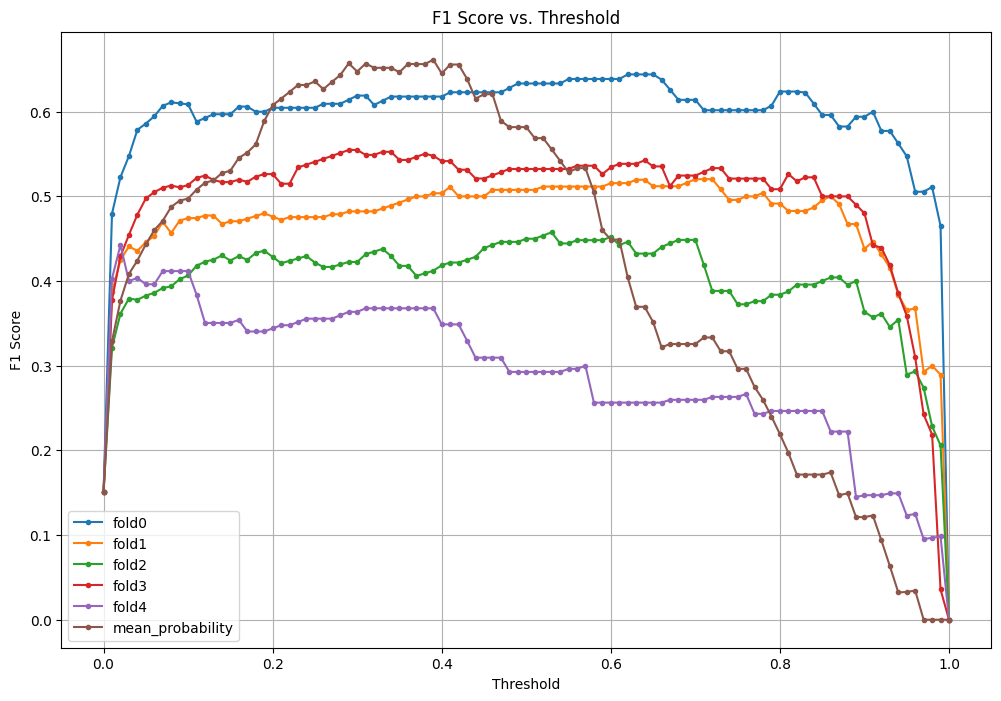
\includegraphics[width=1.0\linewidth]{Images/Chapter3/f1-vs-th-cls}
\caption{نمودار امتیاز \lr{F1} نسبت به آستانه برای \lr{Fold}ها و میانگین آنها}
\label{fig:ch3-f1-vs-th-cls}

\end{figure}


\begin{figure}[h!]
		\centering % <-- added
		\begin{subfigure}{0.45\textwidth}
			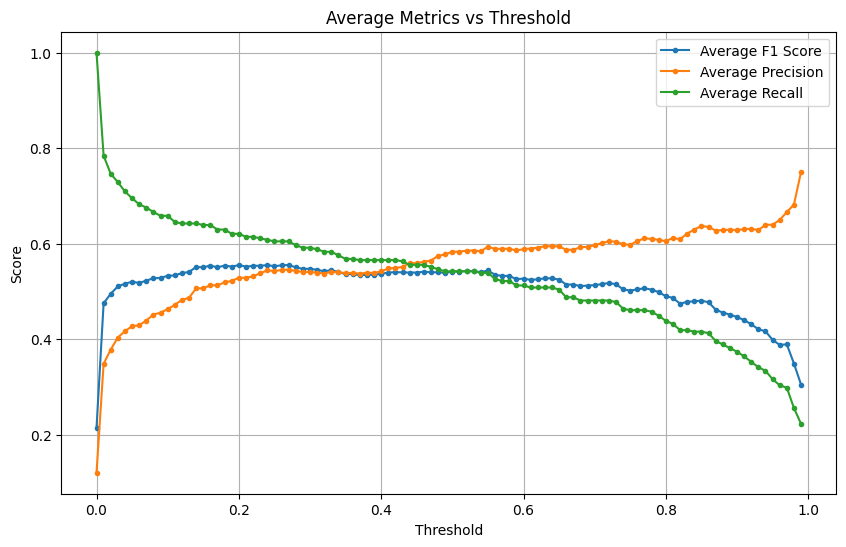
\includegraphics[width=\linewidth]{Images/Chapter3/metrics-cls.png}
			\caption{}
			
			\label{fig:ch3-metrics-cls}
		\end{subfigure}\hfil % <-- 
		\begin{subfigure}{0.45\textwidth}
			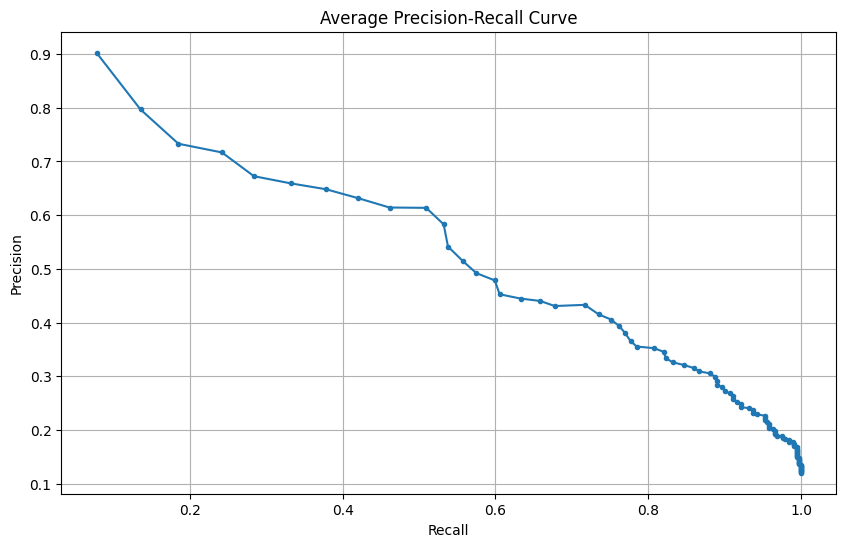
\includegraphics[width=\linewidth]{Images/Chapter3/pr-cls.png}
			\caption{}
			\label{fig:ch3-pr-cls}
		\end{subfigure}\hfil % <-- added
		\caption{نمودارهای سازوکار شورایی روی مجموعه‌داده ارزیابی}
		\label{fig:ch3-metrics and pr cls}
\end{figure}


\begin{figure}[h]
\centering
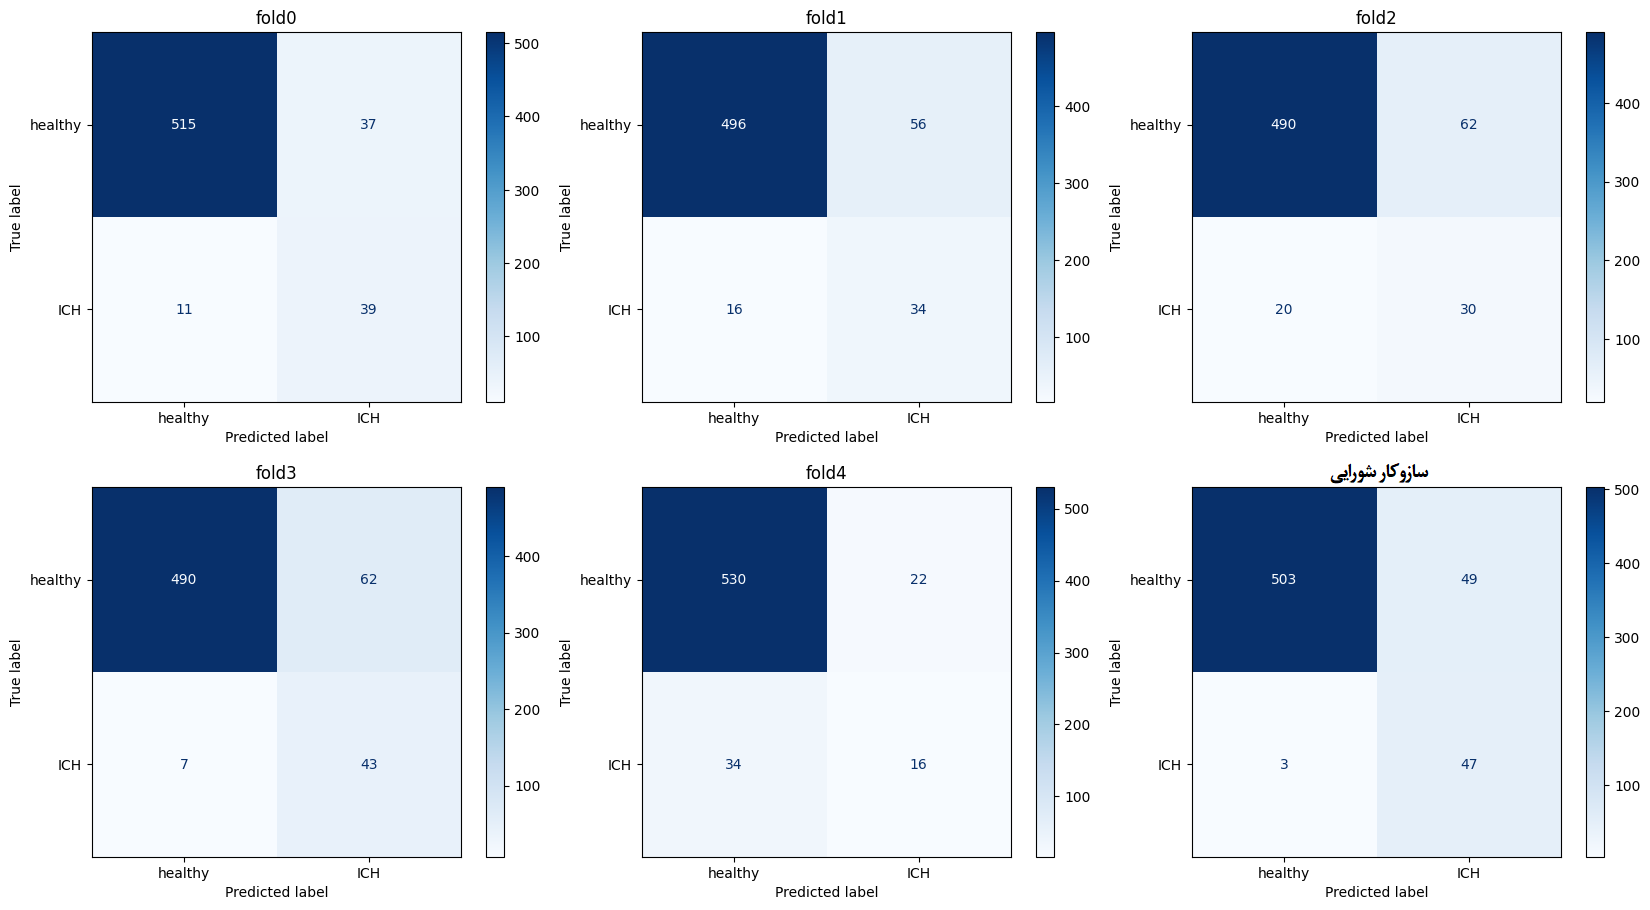
\includegraphics[width=1.0\linewidth]{Images/Chapter3/s-cm}
\caption{ماتریس آشفتگی نتایج برش‌محور}
\label{fig:ch3-s-cm}
\end{figure}


% Please add the following required packages to your document preamble:
% \usepackage{graphicx}
\begin{table}[]
\centering
\caption{نتیجه استفاده از فراپارامترهای بدست آمده از جستجوی شبکه‌ای روی مدل‌های دیگر}
\label{table:ch3-other models cls}
\resizebox{\textwidth}{!}{%
\begin{tabular}{lclllll}
\hline
\multicolumn{1}{c}{\textbf{مدل}} & \textbf{فراپارامتر پیشنهادی} & \textbf{\lr{Sensitivity}} & \textbf{\lr{Specificity}} & \textbf{\lr{Precision}} & \textbf{\lr{F1}} & \textbf{\lr{Accuracy}} \\ \hline
\lr{ResNet 50}      &  $\checkmark$                & $0.94$                 & $0.91$                 & $0.49$          & $0.64$          & $0.91$     \\
\lr{ResNet 50}      &      $\times$           & $0.76$                 & $0.78$                 & $0.23$          & $0.36$          & $0.77$     \\
\lr{VGG-16}         &   $\checkmark$               & $0.92$                 & $0.88$                 & $0.41$          & $0.56$          & $0.88$     \\
\lr{VGG-16}         &       $\times$          & $0.88$                 & $0.76$                 & $0.25$          & $0.39$          & $0.77$     \\
\lr{MobileNet-V2}   &   $\checkmark$               & $0.98$                 & $0.82$                 & $0.33$          & $0.50$          & $0.84$     \\
\lr{MobileNet-V2}   &      $\times$           & $\mathbf{1.00}$           & $\mathbf{0.68}$        & $\mathbf{0.22}$ & $\mathbf{0.36}$ & $0.71$     \\
\lr{Inception-V3}   &   $\checkmark$               & $0.64$                 & $0.90$                 & $0.36$          & $0.46$          & $0.88$     \\
\lr{Inception-V3}   &     $\times$            & $0.88$                 & $0.78$                 & $0.27$          & $0.41$          & $0.79$    
\\ \hline
\end{tabular}%
}
\end{table}


\subsection{نتایج بیمارمحور}

طبقه‌بندی بیمارمحور خونریزی درون‌جمجمه‌ای بر اساس پیش‌بینی‌های برش‌محور انجام شده است. یک بیمار در صورتی دارای خونریزی درون‌جمجمه‌ای در نظر گرفته می‌شود اگر حداقل یک برش از سی‌تی‌اسکن او دارای علائم خونریزی شناسایی شود. نتایج به‌دست‌آمده نشان می‌دهند که مدل 
\lr{ResNet50}
 در بررسی بیمارمحور سی‌تی‌اسکن‌ها، با استفاده از روش شورایی، به 
 \lr{Sensitivity}
  برابر با
   $1.00$، 
   \lr{Specificity}
برابر با
     $0.80$، \lr{Precision}
      برابر با
       $0.75$،
        امتیاز
         \lr{F1}
          برابر با
           $0.86$
            و 
            \lr{Accuracy}
             برابر با
              $0.88$ 
              دست‌یافته است که از تمامی معیارهای گزارش شده در سایر مطالعات، نتیجه بهتری کسب کرده است.
جدول \ref{tab:patient_level_results} نتایج بیمارمحور مدل \lr{ResNet50} را برای هر مرحله آموزشی نشان می‌دهد.
\autoref{fig:ch3-p-cm}
ماتریس آشفتگی بیمارمحور را نشان می‌دهد که از 16 بیمار در مجموعه ارزیابی قرار داشته‌اند که همه 6 بیمار دارای خونریزی درست تشخیص داده شده‌اند.

% Please add the following required packages to your document preamble:
% \usepackage{graphicx}
\begin{table}[]
\centering
\caption{نتایج بیمارمحور مدل \lr{ResNet50}
برای آستانه تصمیم‌گیری 
$0.27$}
\label{tab:patient_level_results}
\resizebox{\textwidth}{!}{%
\begin{tabular}{llllll}
\hline
\multicolumn{1}{c}{\textbf{مدل}}          & \textbf{\lr{Sensitivity}} & \textbf{\lr{Specificity}} & \textbf{\lr{Precision}} & \textbf{\lr{F1}}            & \textbf{\lr{Accuracy}}      \\ \hline
\lr{ResNet50 Fold 1}       & $1.00$                 & $0.60$                 & $0.60$               & $0.75$          & $0.75$          \\
\lr{ResNet50 Fold 2}       & $1.00$                 & $0.60$                 & $0.60$               & $0.75$          & $0.75$          \\
\lr{ResNet50 Fold 3}       & $1.00$                 & $0.60$                 & $0.60$               & $0.75$          & $0.75$          \\
\lr{ResNet50 Fold 4}       & $0.83$                 & $0.80$                 & $0.71$               & $0.77$          & $0.81$          \\ \hline
\lr{Kyung et al.}\cite{kyung2022improved} & $0.97$                 & $0.74$                 & $-$                  & $0.84$          & $-$             \\ \hline
\lr{ResNet50 Voting}       & $\mathbf{1.00}$        & $\mathbf{0.80}$        & $\mathbf{0.75}$      & $\mathbf{0.86}$ & $\mathbf{0.88}$
\\ \hline
\end{tabular}%
}
\end{table}
\begin{figure}[h]
\centering
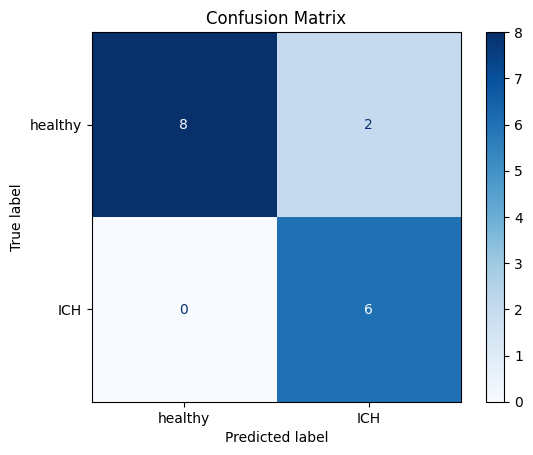
\includegraphics[width=1.0\linewidth]{Images/Chapter3/p-cm}
\caption{ماتریس آشفتگیب یمارمحور سازوکار شورایی}
\label{fig:ch3-p-cm}
\end{figure}


\subsection{تحلیل بیشتر نتایج}

در این بخش، نتایج مرتبط با تفسیرپذیری مدل \lr{ResNet50} از طریق روش‌های \lr{Grad-CAM} و \lr{t-SNE} تحلیل و بررسی می‌شوند.

\subsubsection{تحلیل \lr{Grad-CAM}}

روش 
\lr{Gradient-weighted Class Activation Mapping}
(\lr{Grad-CAM})
 به‌عنوان یک ابزار قدرتمند برای تفسیر مدل‌های شبکه عصبی عمیق استفاده می‌شود. این روش به ما اجازه می‌دهد تا ببینیم کدام بخش‌های تصویر ورودی، بیشتر در تصمیم‌گیری مدل تأثیر داشته‌اند. در این پروژه، از روش
 \lr{Grad-CAM}
  برای افزایش تفسیرپذیری مدل‌های طبقه‌بندی به کمک ایجاد تصویر استفاده شده است که نواحی مهم برش‌های سی‌تی‌اسکن که منجر به تشخیص خونریزی توسط مدل شده‌اند را مشخص می‌‌کند.  
  \autoref{fig:ch3-gradcam} 
  نمونه‌ای از این نقشه‌های حرارتی را نشان می‌دهد که به‌وضوح مشخص می‌کند که مدل چگونه نواحی مختلف تصویر را برای تشخیص \lr{ICH} مورد ارزیابی قرار داده است.
\begin{figure}[h]
\centering
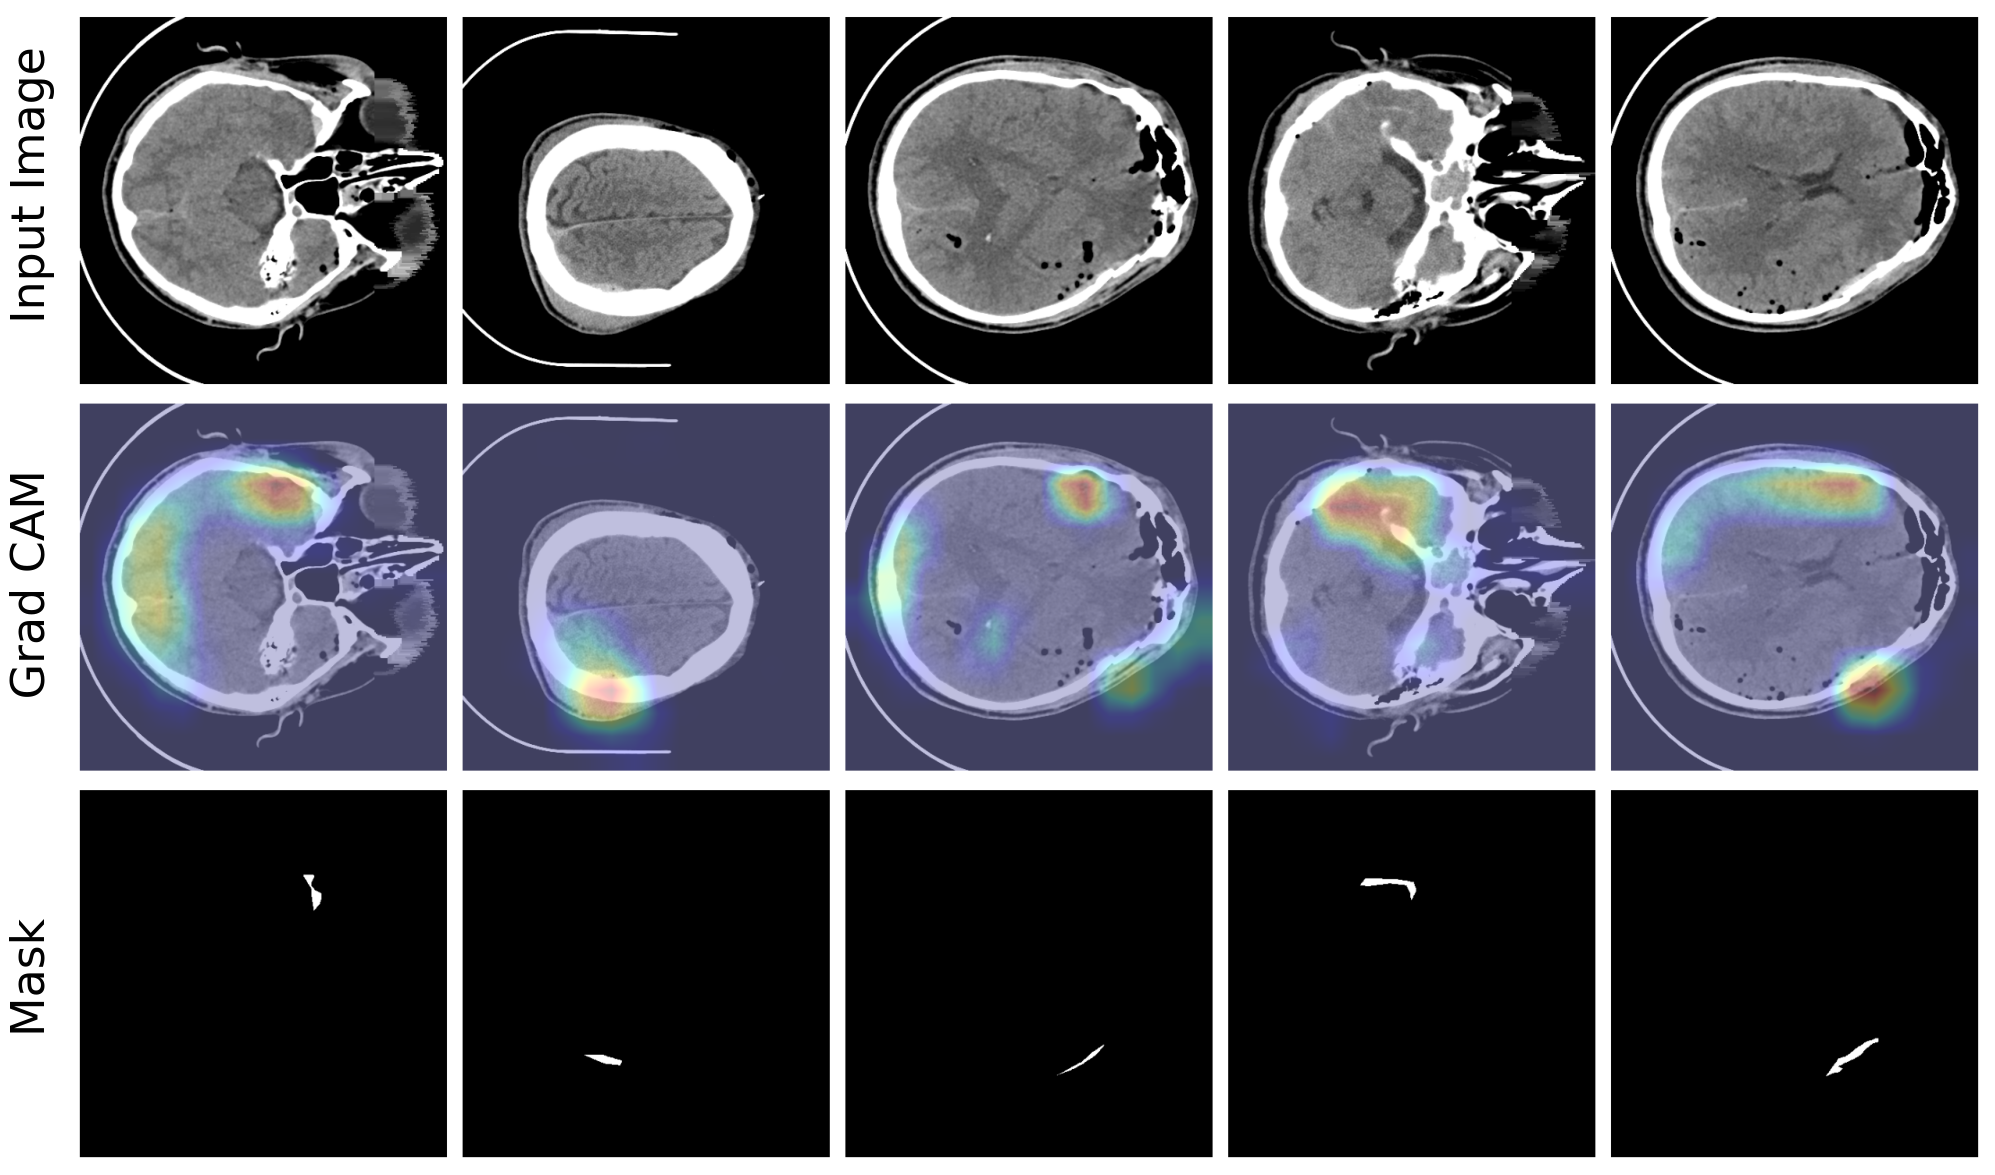
\includegraphics[width=1.0\linewidth]{Images/Chapter3/GradCam}
\caption{چند نمونه از تصاویر تولید شده توسط  \lr{Grad-CAM}}
\label{fig:ch3-gradcam}
\end{figure}

\subsubsection{تحلیل \lr{t-SNE}}

روش
 \lr{t-Distributed Stochastic Neighbor Embedding} (\lr{t-SNE})
  یک روش برای کاهش ابعاد و تجسم داده‌های با ابعاد بالا است. در این پژوهش، از
   \lr{t-SNE}
    برای تجسم توزیع ویژگی‌های استخراج‌شده از مدل \lr{ResNet50} 
    استفاده شده است تا نشان داده شود که آموزش مدل، باعث تولید ویژگی‌هایی شده است که تفکیک‌پذیری برش‌های سالم را از ناسالم زیاد کرده است. 
     \autoref{fig:ch3-tsne}
 نشان‌دهنده توزیع ویژگی‌های استخراجی با روش 
 \lr{t-SNE}
  از تصاویر سی‌تی‌اسکن در فضای دو‌بعدی است که 
  \autoref{fig:ch3-tsne-before}
  پراکندگی ویژگی‌ها از مدل طبقه‌بندی قبل از آموزش آن است و 
    \autoref{fig:ch3-tsne-after}
    بعد از آموزش مدل طبقه‌بندی است. 
      \autoref{fig:ch3-tsne-before}
  به‌وضوح نشان می‌دهد چگونه مدل قادر است تفکیک‌پذیری خطی را برای برش‌های حاوی خونریزی درون‌جمجمه‌ای ایجاد کند. این استخراج ویژگی کمک می‌کند تا دیدگاه بهتری نسبت به نحوه عملکرد مدل در سطح ویژگی‌ها داشته باشیم و نقاط ضعف و قوت آن را بهتر درک کنیم. 
        \autoref{fig:ch3-tsne-other}
نمودار 
\lr{t-SNE}
حاصل از مدل طبقه‌بندی 
\lr{Ganeshkumar}\cite{Ganeshkumar2022Identification}
و همکاران است که نشان می‌دهد مدل به‌دست‌آمده در پژوهش آنها، امکان تفکیک‌پذیری خطی را برای برش‌ها ایجاد نکرده است.

\begin{figure}[h!]
		\centering % <-- added
		\begin{subfigure}{0.33\textwidth}
			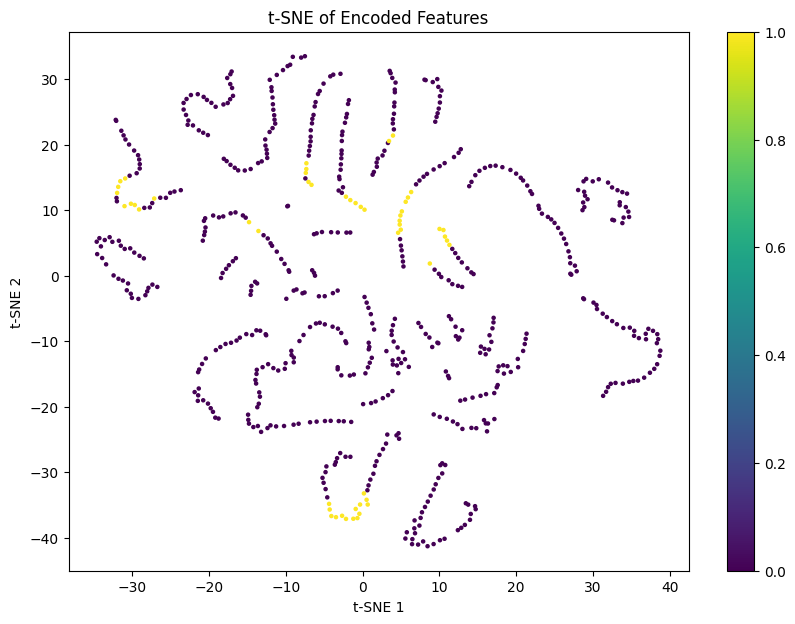
\includegraphics[width=\linewidth]{Images/Chapter3/tsne_vanilla.png}
			\caption{قبل از آموزش}
			\label{fig:ch3-tsne-before}
		\end{subfigure}\hfil % <-- 
		\begin{subfigure}{0.33\textwidth}
			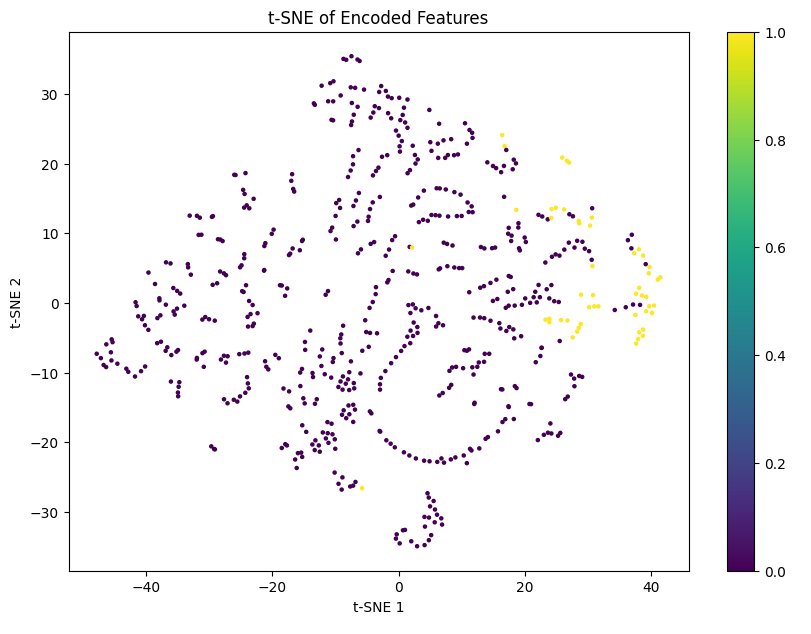
\includegraphics[width=\linewidth]{Images/Chapter3/tsne.png}
			\caption{بعد از آموزش}
			\label{fig:ch3-tsne-after}
		\end{subfigure}\hfil % <-- added
        \begin{subfigure}{0.33\textwidth}
			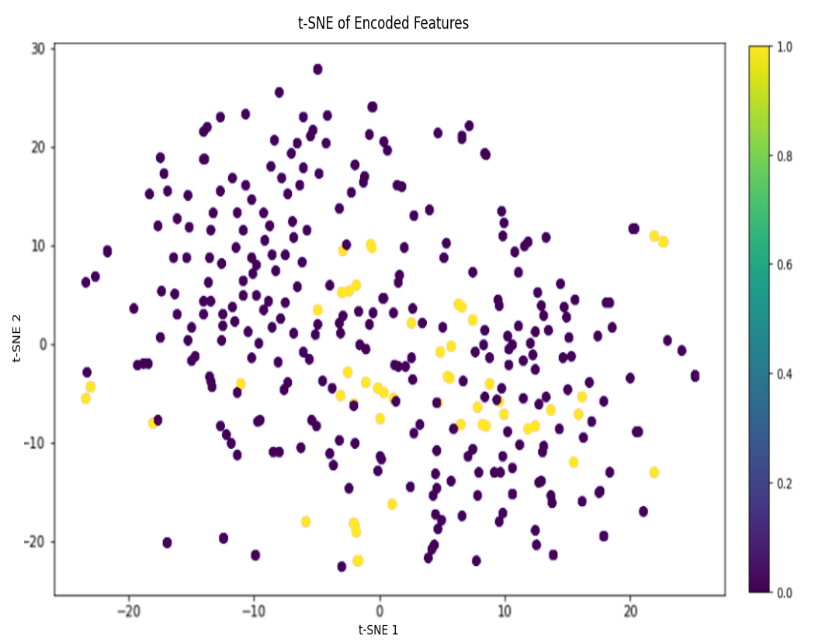
\includegraphics[width=\linewidth]{Images/Chapter3/tsne-other.png}
			\caption{مدل  
			\lr{Ganeshkumar} 
			\cite{Ganeshkumar2022Identification}}
			\label{fig:ch3-tsne-other}
        \end{subfigure}
		\caption{نمودارهای 
		\lr{t-SNE}
		و مقایسه آنها با یکدیگر}
		\label{fig:ch3-tsne}
\end{figure}


\section{نتایج قطعه‌بندی}
در این قسمت به بررسی نتایج حاصل شده از آموزش مدل قطعه‌بندی 
\lr{U-Net}و \lr{PSPNet}
 می‌پردازیم. نتیجه استفاده از جستجوی شبکه‌ای به روی مدل 
 \lr{‎U-Net}
 نشان می‌دهد که مدل با رمزگذار 
 \lr{SE-ResNeXt-101}
که با استفاده از تابع خطا
\lr{ِDice}
آموزش‌دیده و میزان برش‌های دارای خونریزی آن، 5 برابر شده است، بهترین نتیجه را به‌دست‌آورده‌. باتوجه به فراپارامتر‌هایی که در جستجوی شبکه‌ای مدل
 \lr{‎U-Net}
 به‌دست‌آمد، مدل
 \lr{PSPNet}
 آموزش داده شد تا نشان دهیم این فراپارامترها می‌توانند عملکرد مدل‌های قطعه‌بندی را بهبود بخشند. 
 \autoref{fig:ch3-seg-training-graph}
 منحنی‌های مربوط به آموزش مدل روی 
 \lr{Fold 1}
را نشان می‌دهد که در آن 
 \lr{\texttt{Original test without post-process}}،
 مربوط به مجموعه‌داده ارزیابی است که از مدل طبقه‌بندی عبور داده نشده است و عملیات پس‌پردازش به روی آن انجام نشده است.
 منحنی 
 \lr{\texttt{Original test with post-process}}
 مربوط به مجموعه‌داده ارزیابی است که از مدل طبقه‌بندی عبور داده نشده‌ است؛ اما عملیات پس‌پردازش به روی آن انجام شده است.
منحنی 
 \lr{\texttt{Reduced test with post-process}}
 مربوط به مجموعه‌داده ارزیابی است که از مدل طبقه‌بندی عبور داده شده و عملیات پس‌پردازش به روی آن انجام شده است.
 همان‌طور که از نمودارهای مربوط به معیار
 \lr{IoU}
 در 
 \autoref{fig:ch3-seg-IoU}
 و معیار 
 \lr{Dice}
  در 
  \autoref{fig:ch3-seg-Dice}
  مشخص است،‌ پس‌پردازش پیشنهادی و روش دومرحله‌ای هرکدام باعث بهبود چشمگیر نتایج مدل شبکه عصبی شده‌اند.
 
 \begin{figure}[h!]
 		\centering % <-- added
 		\begin{subfigure}{0.49\textwidth}
 			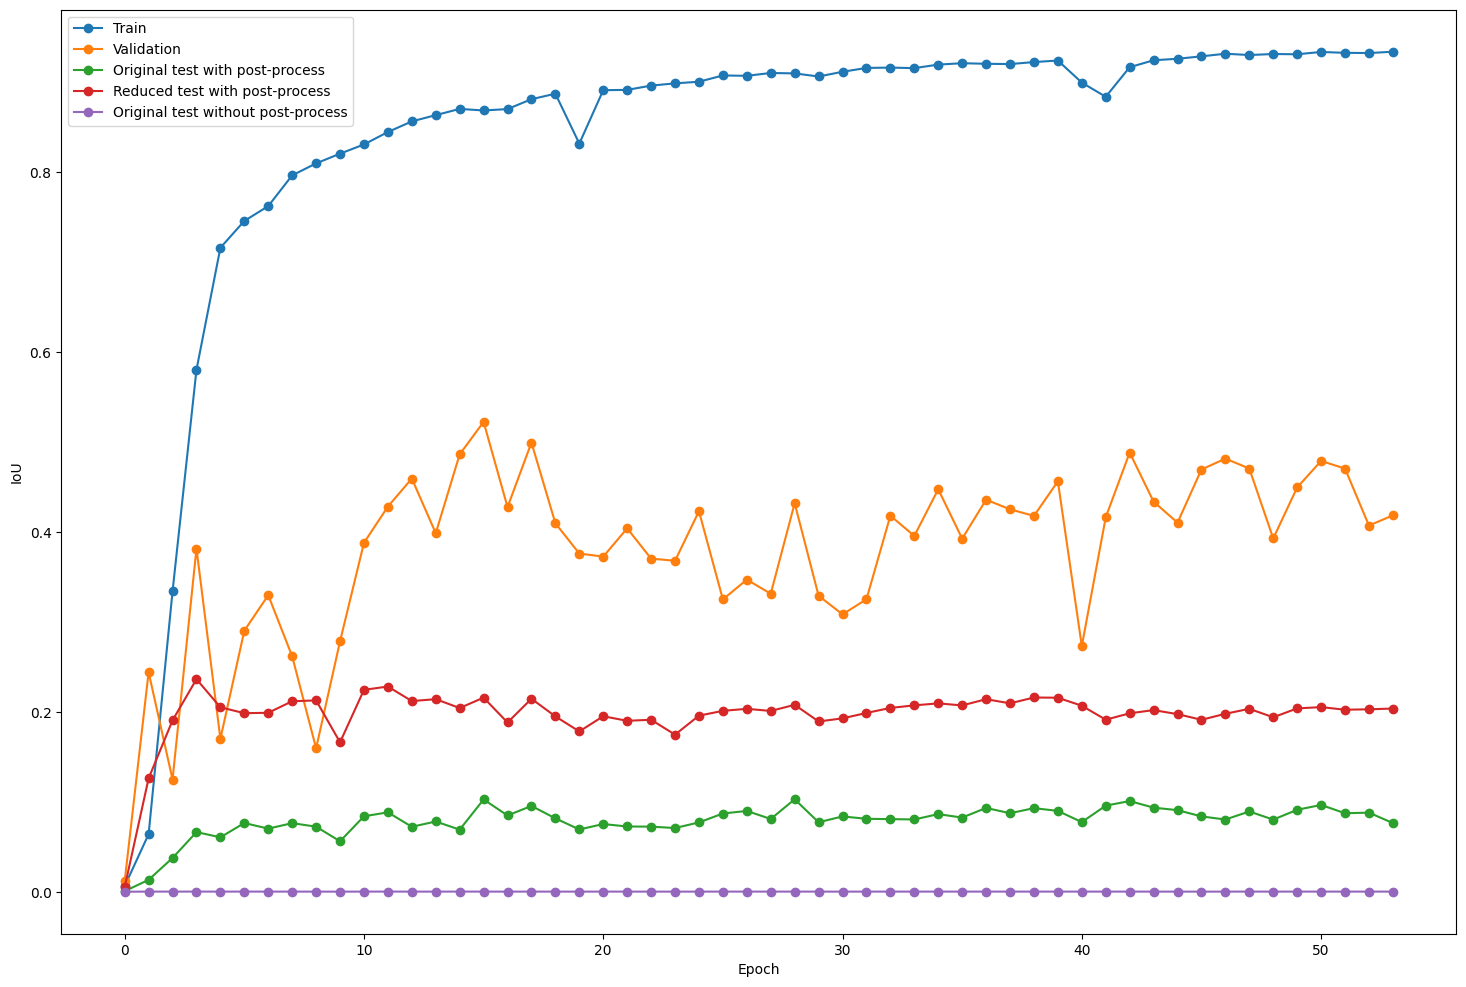
\includegraphics[width=\linewidth]{Images/Chapter3/seg-IoU-metrics.png}
 			\caption{\lr{IoU}}
 			\label{fig:ch3-seg-IoU}
 		\end{subfigure}\hfil % <-- 
 		\begin{subfigure}{0.49\textwidth}
 			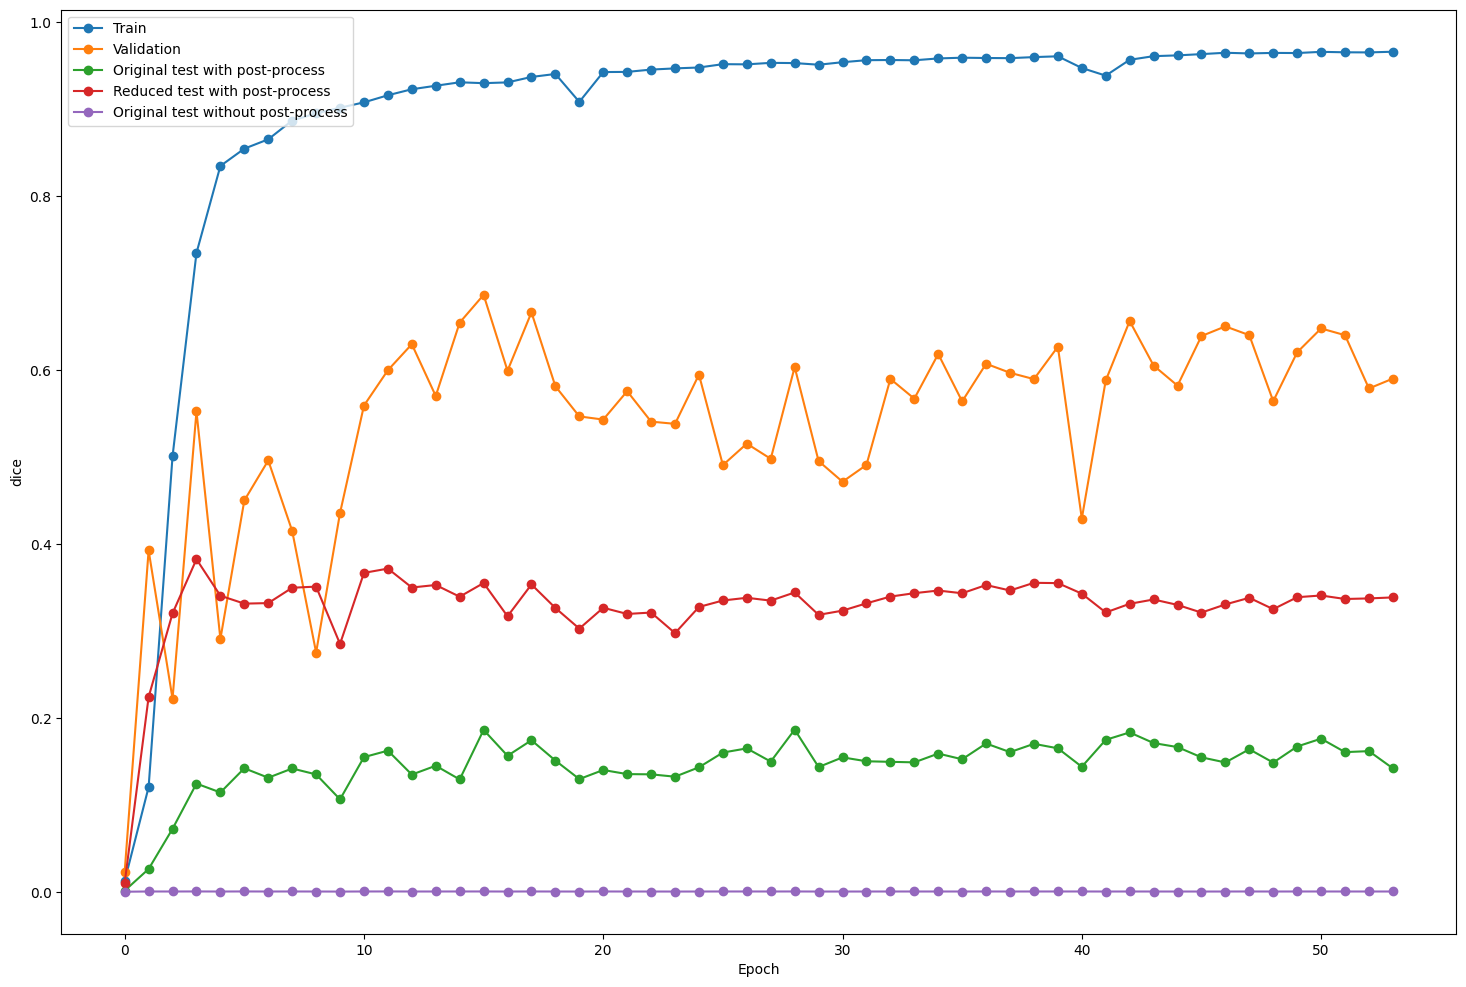
\includegraphics[width=\linewidth]{Images/Chapter3/seg-Dice-metrics.png.png}
 			\caption{\lr{Dice}}
 			\label{fig:ch3-seg-Dice}
 		\end{subfigure}\hfil % <-- added
 		\caption{یک نمونه از عملکرد روش پیشنهادی و پس‌پردازش در فرایند آموزش }
 		\label{fig:ch3-seg-training-graph}
 \end{figure}
 
 با درنظرگرفتن کمترین مقدار تابع خطا، بهترین
 \lr{Epoch}
 هر 
 \lr{Fold}
 انتخاب می‌شود و پس از آن برای تنظیم متغیرهای مربوط به سازوکار شورا، نمودارهای 
 \lr{ِIoU}
 و 
 \lr{Dice}
 نسبت به آستانه‌های متفاوت رسم می‌شود و بهترین آستانه به دست می‌آید.
 
 \autoref{table:ch3-seg-results}
 نتایج 
 \lr{ّFold}ها،
 روش شورایی و تحقیقات گذشته را نشان می‌دهد. همان‌طور که مشخص است روش مذکور توانسته معیار
 \lr{Dice}
 را نسبت به مطالعات پیشین بهبود ببخشید درحالی‌که مقدار 
 \lr{IoU}
 آن نیز به‌صورت کلی از آنها بهتر است.

 \begin{table}[]
 \centering
 \caption{نتایج قطعه‌بندی تصاویر سی‌تی‌اسکن}
 \label{table:ch3-seg-results}
  \adjustbox{width=0.8\columnwidth,max totalheight=\textheight, keepaspectratio}{
 \begin{tabular}{rllll}
 \hline
 \textbf{مدل} & \textbf{} & \multicolumn{1}{r}{\textbf{\lr{IoU}}}  & \textbf{} & \multicolumn{1}{r}{\textbf{\lr{Dice}}} \\ \cline{2-5}
                                                  & عادی      & دو مرحله‌ای    & عادی      & دو مرحله‌ای    \\ \hline
 \lr{U-Net Fold 0}                                                       & $0.12$      & $0.21$          & $0.21$      & $0.35$          \\
 \lr{PSPNet Fold 0}                                                       & $0.18$      & $0.22$          & $0.31$      & $0.36$          \\
 \lr{U-Net Fold 1}                                                       & $0.17$      & $0.20$          & $0.29$      & $0.34$          \\
 \lr{PSPNet Fold 1}                                                       & $0.17$      & $0.21$          & $0.29$      & $0.35$          \\
 \lr{U-Net Fold 2}                                                       & $0.06$      & $0.20$          & $0.12$      & $0.33$          \\
 \lr{PSPNet Fold 2}                                                       & $0.11$      & $0.16$          & $0.20$      & $0.28$          \\
 \lr{U-Net Fold 3}                                                       & $0.19$      & $0.19$          & $0.16$      & $0.32$          \\
 \lr{PSPNet Fold 3}                                                       & $0.20$      & $0.23$          & $0.34$      & $0.37$          \\
 \lr{U-Net Fold 4}                                                       & $0.09$      & $0.19$          & $0.16$      & $0.33$          \\ 
 \lr{PSPNet Fold 4}                                                       & $0.16$      & $0.21$          & $0.27$      & $0.35$          \\
  \hline
 \lr{U-Net Hssayeni}\cite{hssayeni2020intracranial}                                                          & $0.22$      & -             & $0.32$      & -             \\
 \lr{U-Net Neethi}\cite{neethi2022stroke}                                                          & $0.20$      & -             & $0.35$      & -             \\ \hline
 \lr{U-Net} شورایی
                                                        & $0.17$      & $0.22$ & $0.29$      & $0.36$\\
\lr{PSPNet} شورایی
                                                        & $0.20$      & \textbf{$0.23$} & $0.34$      & \textbf{$0.38$}
 \\ \hline
 \end{tabular}%
 }
 \end{table}
 
 
 
 
 
 \autoref{fig:dice-th-seg-unet} و \autoref{fig:dice-th-seg-psp}
 نتایج 
  \lr{ِIoU}
  و 
  \lr{Dice}
 را به‌ازای آستانه‌های متفاوت برای دو مدل
 \lr{U-Net} و \lr{PSPNet}
 نشان می‌دهند. همان‌طور که مشخص است، میانگین عملکرد مدل‌ها به روی زیرمجموعه اعتبارسنجی که توزیع برش‌های آن، مشابه با توزیع برش‌ها در زیرمجموعه ارزیابی است، بسیار بیشتر از نتایج به‌دست‌آمده به روی زیرمجموعه ارزیابی است. علت اصلی این تفاوت، در توزیع مکانی خونریزی درون‌جمجمه‌ای موجود در زیرمجموعه ارزیابی نسبت به بقیه زیر‌مجموعه‌ها است که در 
 \autoref{fig:heatmaps}
 این تفاوت توزیع مشخص است. 
 \lr{Hssayeni}\cite{hssayeni2020intracranial} 
 و همکاران، در پژوهشی که نتایج آن در
 \autoref{table:ch3-seg-results}
 آورده شده است، نتایج خود را از میانگین گرفتن از نتایج به‌دست‌آمده از هر
 \lr{Fold}
 گزارش کرده‌اند؛ بنابراین اگر این معیار را برای ارزیابی نتایج روش دومرحله‌ای در نظر بگیریم، این روش بهبود قابل‌توجهی در معیارهای قطعه‌بندی ایجاد کرده است.
 

   \begin{figure}[h!]
   		\centering % <-- added
   		\begin{subfigure}{0.49\textwidth}
   			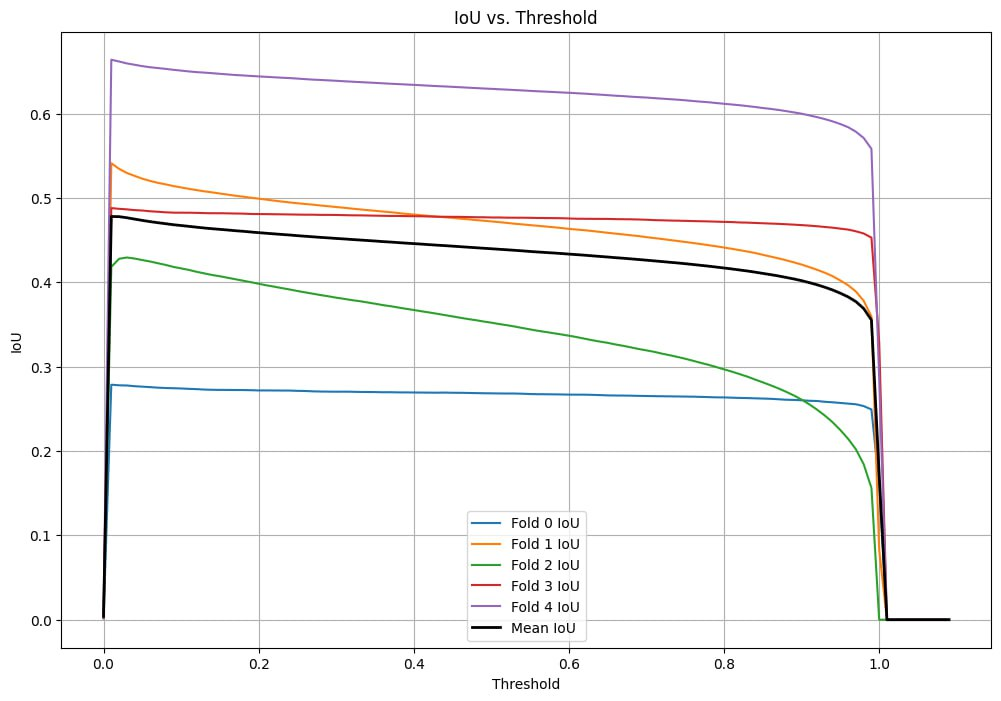
\includegraphics[width=\linewidth]{Images/Chapter3/IoU-th-seg-psp.jpg}
   			\caption{\lr{IoU}}
   			\label{fig:ch3-seg-IoU-unet}
   		\end{subfigure}\hfil % <-- 
   		\begin{subfigure}{0.49\textwidth}
   			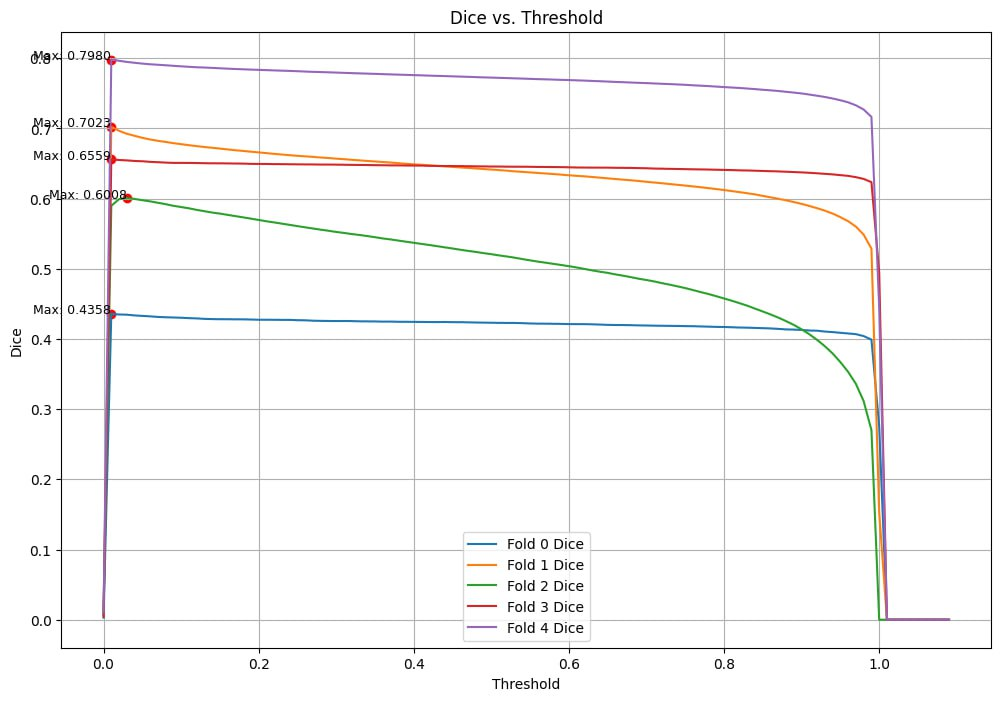
\includegraphics[width=\linewidth]{Images/Chapter3/Dice-th-seg-psp.jpg}
   			\caption{\lr{Dice}}
   			\label{fig:ch3-seg-Dice-unet}
   		\end{subfigure}\hfil % <-- added
 \caption{نتایج مدل
 \lr{U-Net}
 به‌ازای آستانه‌های متفاوت}
   		\label{fig:dice-th-seg-unet}
   \end{figure}
   
 
  \begin{figure}[h!]
  		\centering % <-- added
  		\begin{subfigure}{0.49\textwidth}
  			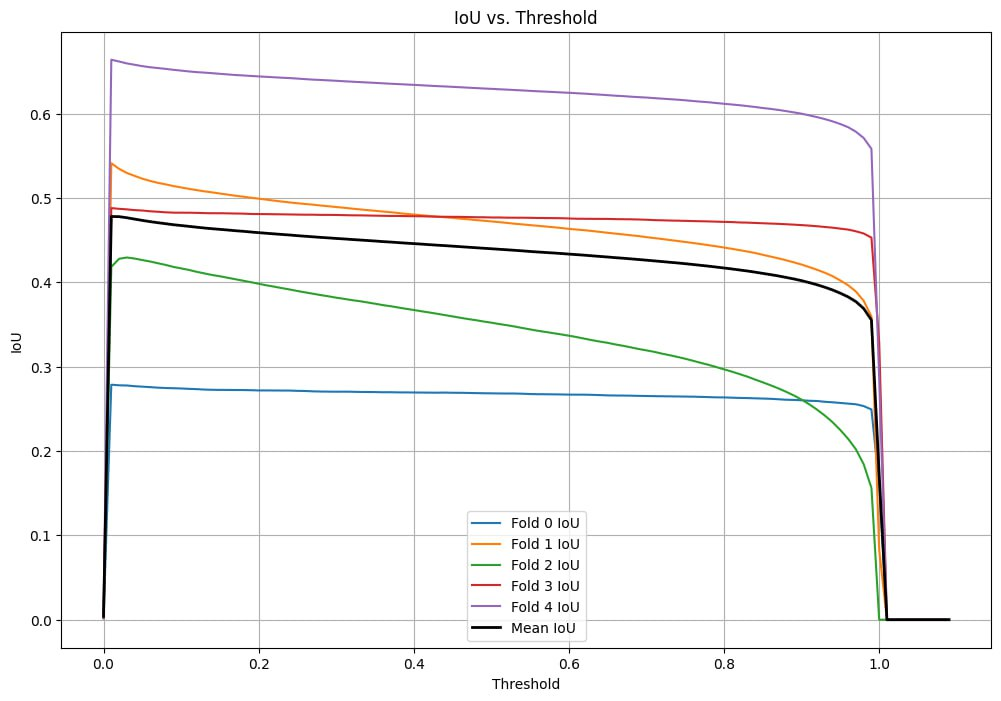
\includegraphics[width=\linewidth]{Images/Chapter3/IoU-th-seg-psp.jpg}
  			\caption{\lr{IoU}}
  			\label{fig:ch3-seg-IoU-psp}
  		\end{subfigure}\hfil % <-- 
  		\begin{subfigure}{0.49\textwidth}
  			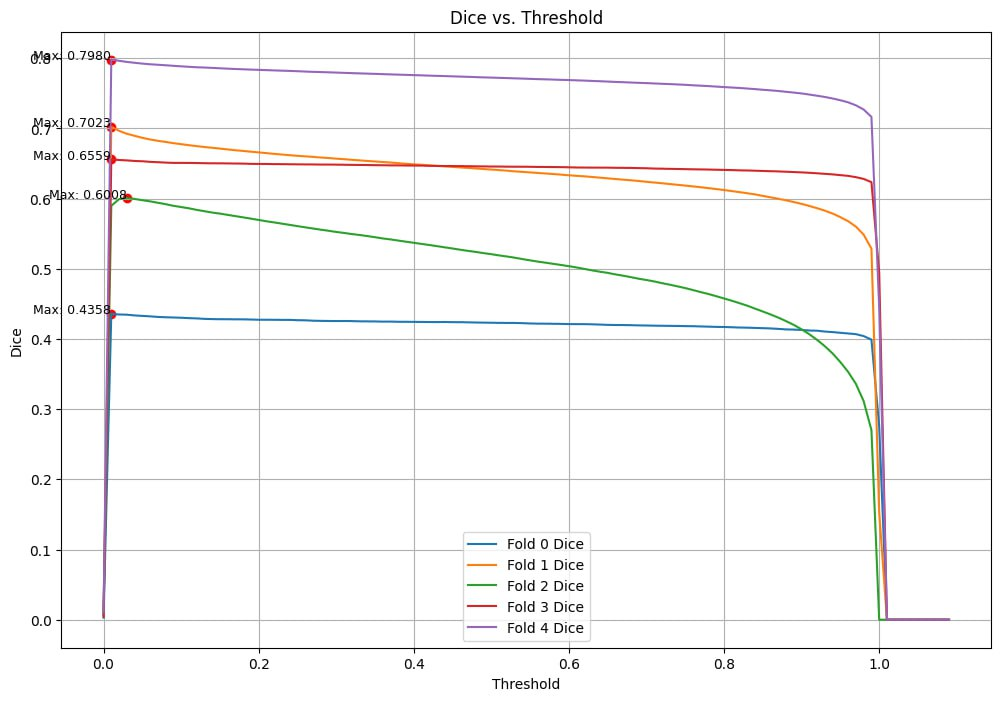
\includegraphics[width=\linewidth]{Images/Chapter3/Dice-th-seg-psp.jpg}
  			\caption{\lr{Dice}}
  			\label{fig:ch3-seg-Dice-psp}
  		\end{subfigure}\hfil % <-- added
\caption{نتایج مدل
\lr{PSPNet}
به‌ازای آستانه‌های متفاوت}
  		\label{fig:dice-th-seg-psp}
  \end{figure}
  
\autoref{fig:results-seg}
چند عملکرد مدل را در پیش‌بینی خونریزی در چند نمونه برش نشان می‌دهد. از بررسی این تصاویر مشخص است که مدل شبکه عصبی در پیش‌بینی خونریزی در برش‌ها دچار زیرقطعه‌بندی 
\lr{Under Segmentation}
و لازم است تا با اضافه کردن یک تابع هزینه مناسب یا یک پس‌پردازش این مسئله رفع شود، از طرف دیگر با بررسی ستون‌های موجود در
\autoref{fig:results-seg}،
مشخص است که در ستون آخر با وجود اینکه مساحت خونریزی زیاد بوده؛ اما قطعه‌بندی به صورت درستی انجام نشده است. علت به وجود آمدن این مشکل این است که خونریزی درون‌‌جمجمه‌ای، در زمان ابتدایی وقوع حادثه بافت تیره‌تری نسبت به بقیه قسمت‌های مغز دارد و با گذر زمان رنگ این ضایعه نسبت به بقیه اجزای مغز روشن‌تر می‌شود؛ بنابراین با توجه به اینکه تصویر سی‌تی‌اسکن در چه زمانی گرفته شود رنگ این ضایعه متفاوت است. مشکل موجود در مجموعه‌داده 
\lr{PhysioNet}
نبود تعداد کافی برش دارای خونریزی به رنگ تیره می‌باشد و در ادامه آن مدل‌های مبتنی بر شبکه عصبی پیچشی حساسیت بیشتری به بافت تصویر دارند تا شکل ضایعه موجود در تصویر بنابراین مدل پیشنهادی 
\lr{Bias}
بیشتری دارد تا خونریزی‌هایی با رنگ روشن را بهتر تشخیص دهد.



\begin{figure}[h]
\centering
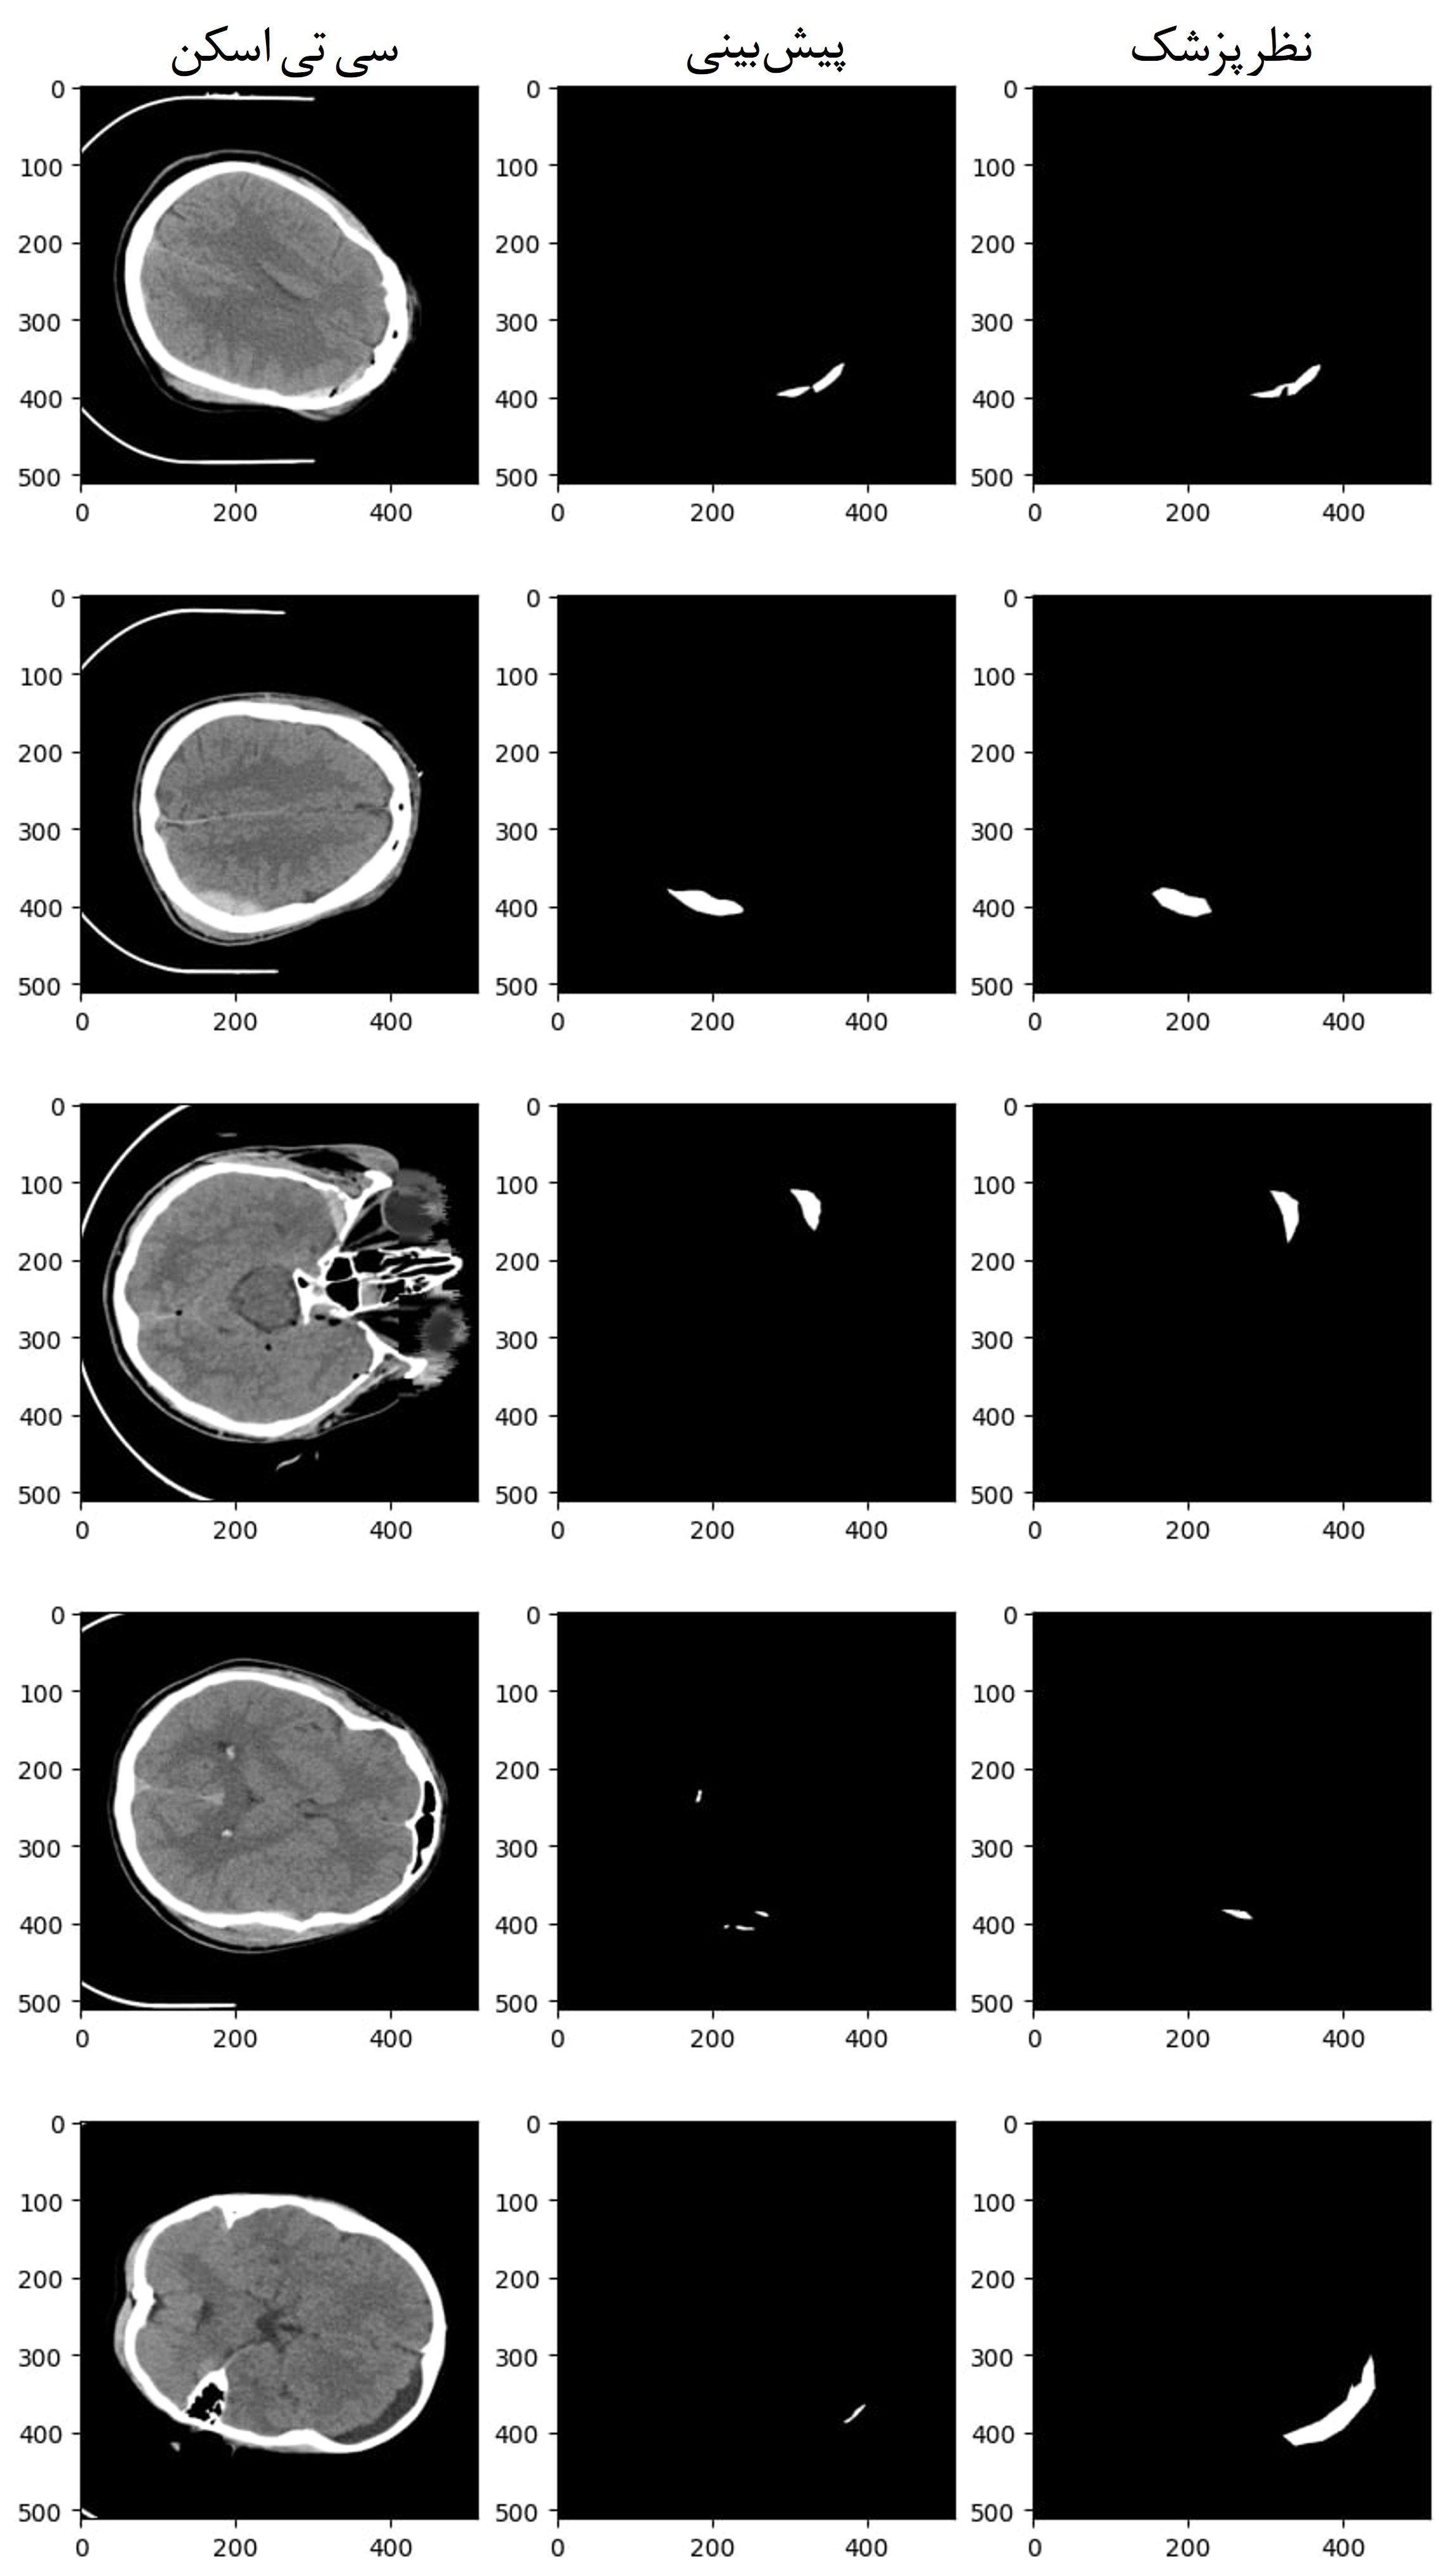
\includegraphics[width=0.85\linewidth]{Images/Chapter3/results.jpg}
\caption{نمونه عملکرد مدل در پیش‌بینی تصاویر سی‌تی‌اسکن}
\label{fig:results-seg}
\end{figure}
  